\appendix

\chapter{Technical Implementation Reference}

\setlength{\parindent}{1em}

This appendix collects technical material that supports, but would interrupt, the
main text: the architecture summary, the full extraction prompt and schema, the
security implementation, the user-interface gallery, and a record of engineering
challenges and decisions.

\section{System Architecture Overview}

\subsection{Architecture Components}

MiPay is a three-tier, three-container system. The \textbf{presentation tier} is a
Flutter application; the \textbf{application tier} is a FastAPI service hosting the
Whisper model in-process and the business logic; and the \textbf{data and
inference tier} comprises PostgreSQL for persistence and an Ollama server for the
language model. Table~\ref{tab:stack-summary} summarizes the stack.

\begin{table}[H]
\centering
\caption{Technology stack summary.}
\label{tab:stack-summary}
\small
\renewcommand{\arraystretch}{1.25}
\begin{tabularx}{\textwidth}{l X}
\toprule
\textbf{Concern} & \textbf{Choice} \\
\midrule
Mobile client & Flutter (Dart), Riverpod state management, Dio HTTP, go\_router \\
Backend & FastAPI (Python 3.11+), async SQLAlchemy 2.0, Pydantic v2 \\
Database & PostgreSQL 16, Alembic migrations \\
Speech-to-text & faster-whisper (CTranslate2), model \texttt{small}, \texttt{int8} \\
Extraction LLM & Qwen2.5-7B-Instruct via Ollama, schema-constrained decoding \\
Dates & \texttt{dateparser} (ar/en), with dialect pre-mapping \\
Auth & JWT (HS256), bcrypt password hashing \\
Deployment & Docker Compose (\texttt{api}, \texttt{postgres}, \texttt{ollama}) \\
\bottomrule
\end{tabularx}
\end{table}

\section{Frontend Architecture}

\subsection{Technology Stack}

The client uses Flutter for cross-platform UI, Riverpod~\cite{riverpod} for
reactive state, Dio for HTTP with a token-refresh interceptor, \texttt{record} for
audio capture (AAC/m4a, 16\,kHz mono), \texttt{flutter\_secure\_storage} for
tokens, \texttt{fl\_chart} for the dashboard donut chart, and
\texttt{flutter\_localizations}/\texttt{intl} with ARB files for bilingual
localization.

\subsection{State Management Strategy}

State is organized into Riverpod providers: an auth controller exposing an
authenticated/unauthenticated state; a Dio provider configured with the
auth interceptor; a recording controller implementing the
\texttt{idle\,$\rightarrow$\,recording\,$\rightarrow$\,uploading\,$\rightarrow$\,processing\,$\rightarrow$\,result}
state machine; a paginated transactions provider invalidated on every mutation;
a monthly summary provider; and a settings provider holding locale and default
currency, persisted locally and synced to the API.

\subsection{Key Components and Implementation}

The hero screen is the record screen, whose large microphone button drives the
recording state machine and surfaces staged progress text. The confirmation
screen renders one editable card per extracted record and commits them through the
atomic batch endpoint. The transactions screen groups records by day with month,
category, and type filters; the dashboard screen presents three stat cards and the
category donut chart; and the settings screen switches language (including
right-to-left layout) instantly.

\section{Backend Architecture}

\subsection{Service Layer Implementation}

The backend separates concerns into routers (\texttt{api/v1/}), Pydantic schemas,
SQLAlchemy models, and a service layer. The service layer is where the AI logic
lives: \texttt{stt.py} (the Whisper singleton), \texttt{extraction.py} (the
constrained Ollama client, schema, and prompt), \texttt{postprocess.py} (the
deterministic layer), \texttt{audio.py} (ffmpeg conversion and cleanup), and
\texttt{voice\_pipeline.py} (the orchestrator with \texttt{process\_audio} and
\texttt{process\_text} entry points sharing one extraction core).

\subsection{Data Access and API Integration}

Data access uses async SQLAlchemy sessions injected as FastAPI dependencies. Every
transaction and summary query is filtered by the authenticated user's identifier.
The Whisper model is loaded once in the application lifespan handler and held on
application state; the CPU-bound \texttt{transcribe} call is dispatched to a worker
thread so the event loop remains free.

\section{Core Service / Engine: the Extraction Prompt}

\subsection{System Prompt}

Listing~\ref{lst:prompt} reproduces the extraction system prompt. The source uses
native Arabic script for the mapping examples; here those Arabic tokens are shown
in transliteration (English only), but the rules are otherwise verbatim.

\begin{lstlisting}[caption={Extraction system prompt (Arabic example tokens transliterated).}, label={lst:prompt}]
You are a financial transaction extraction engine for a personal finance app.
The user message is a voice-note transcript in Arabic, English, or a mix of both.
Return JSON of the form {"transactions": [ ... ]} following the provided schema.

- A single transcript may describe MULTIPLE transactions. Emit one object per
  distinct transaction in the "transactions" array, in the order spoken. Split
  whenever there are separate amounts or separate items/recipients. A single item
  with one amount is ONE transaction.
- If the transcript describes no transaction at all, return {"transactions": []}.

Per-transaction field rules:
- "transaction_type": "expense" if the user paid/spent/bought, "income" if the
  user received/earned/was paid/was sent money. null only if impossible to tell.
- "amount": the numeric amount only. Convert spelled-out numbers in either
  language ("fifty", "khamsin" -> 50; "miya wa khamsin" -> 150). Keep as spoken.
- "currency": ISO code of the spoken currency. Map words: riyal -> SAR (unless
  Qatari -> QAR or Omani -> OMR), dollar/bucks -> USD, gineh (Egyptian) -> EGP,
  dirham -> AED (unless Moroccan -> MAD), dinar -> KWD/JOD/BHD/IQD/LYD/TND by
  national context, euro -> EUR, lira (Lebanese) -> LBP, (Syrian) -> SYP.
  If no currency is spoken, return null.
- "category": pick the single best value from the schema enum (groceries,
  restaurants, transport, fuel, bills, rent, health, salary, transfer_in, ...).
  If nothing fits, use "other".
- "name": the merchant, store, person, or a 2-4 word description, in the language
  spoken. null if not mentioned.
- "date_text": copy the EXACT date phrase from the transcript ("yesterday",
  "ams", "yom el-gomaa", "last week", "3 March"). Do NOT resolve it to a date.
  null if no date phrase is present.
- "confidence": "high" if amount and type are explicit; "medium" if inferred;
  "low" if the utterance barely describes a transaction.
- Never invent values. Prefer null over guessing.
\end{lstlisting}

\subsection{Few-Shot Examples}

Eight examples are sent as alternating user/assistant messages before the real
transcript, teaching the model to wrap single transactions in a list, to split
compound utterances into several objects, and to return an empty list when no
transaction is described. Listing~\ref{lst:fewshot} shows two representative
examples (Arabic transliterated).

\begin{lstlisting}[language=json, caption={Two representative few-shot examples.}, label={lst:fewshot}]
user:      i bought a coffee 50 bucks and a croissant 100 bucks and dad gave me 200
assistant: {"transactions":[
  {"transaction_type":"expense","amount":50,"currency":"USD","category":"restaurants","name":"coffee","date_text":null,"confidence":"high"},
  {"transaction_type":"expense","amount":100,"currency":"USD","category":"restaurants","name":"croissant","date_text":null,"confidence":"high"},
  {"transaction_type":"income","amount":200,"currency":"USD","category":"transfer_in","name":"father","date_text":null,"confidence":"high"}]}

user:      [Arabic] dafact khamsin riyal cala l-baqala min Carrefour ams
assistant: {"transactions":[
  {"transaction_type":"expense","amount":50,"currency":"SAR","category":"groceries","name":"Carrefour","date_text":"ams","confidence":"high"}]}
\end{lstlisting}

\section{Security Implementation}

\subsection{Authentication and Authorization}

Authentication issues a 30-minute HS256 access token and a 30-day refresh token.
Refresh tokens are rotated on every use and carry a \texttt{token\_version} that is
incremented to revoke all sessions. Passwords are hashed with bcrypt. A FastAPI
dependency extracts and validates the bearer token and yields the current user;
every data query filters on that user's identifier, so cross-user access is
impossible by construction (FR-13).

\subsection{API Security and Data Protection}

All errors are rendered in a uniform \texttt{\{error:\{code,message\}\}} envelope
via a global exception handler, avoiding leakage of internal details. Secrets
(JWT key, database URL) are supplied only through environment variables.

\subsection{Privacy and Compliance}

The system's strongest privacy property is structural: uploaded audio is converted,
transcribed, and then deleted immediately (NFR-04); only the transcript is retained,
attached to its transaction for traceability. No audio or text is sent to any third
party, since both models are self-hosted. This design aligns with data-minimization
principles such as those of the GDPR~\cite{voigt2017gdpr}: the system collects and
retains only what it needs, and the most sensitive artifact (the voice recording)
is never persisted.

\section{Platform Features and User Interface}

\subsection{Core Functionality}

The platform supports three input modes (voice, typed text, manual) converging on a
single confirm-and-save path; full CRUD over transactions; filtered listing; a
monthly dashboard; and instant Arabic/English switching with right-to-left support.

\subsection{User Interface Screenshots}

The figures below catalogue the application screens. Each is sourced as a
\texttt{.jpg} screenshot (see the figure guide).

\begin{figure}[H]
    \centering
    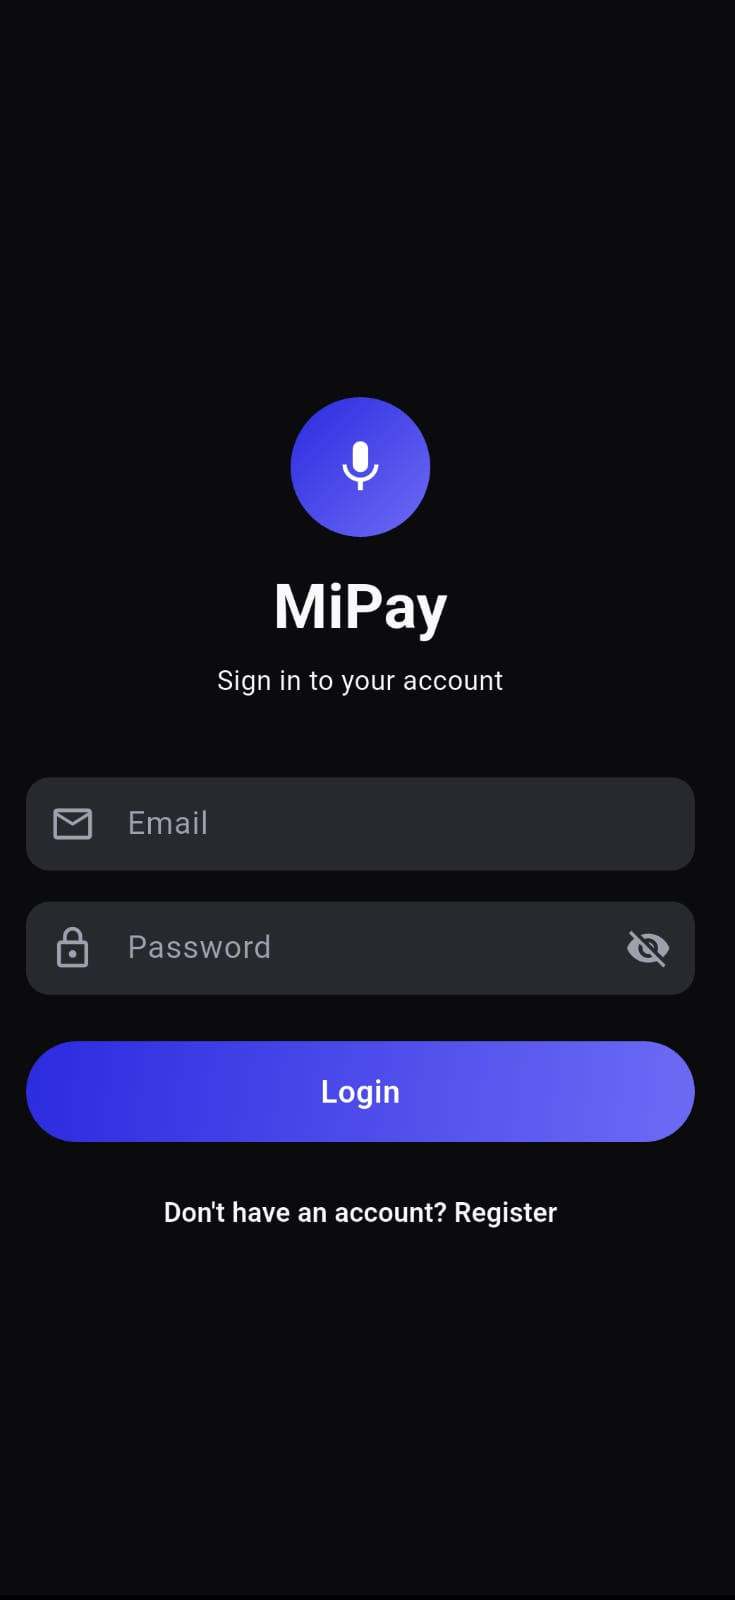
\includegraphics[width=0.32\textwidth]{figures/ui_login.jpg}\hfill
    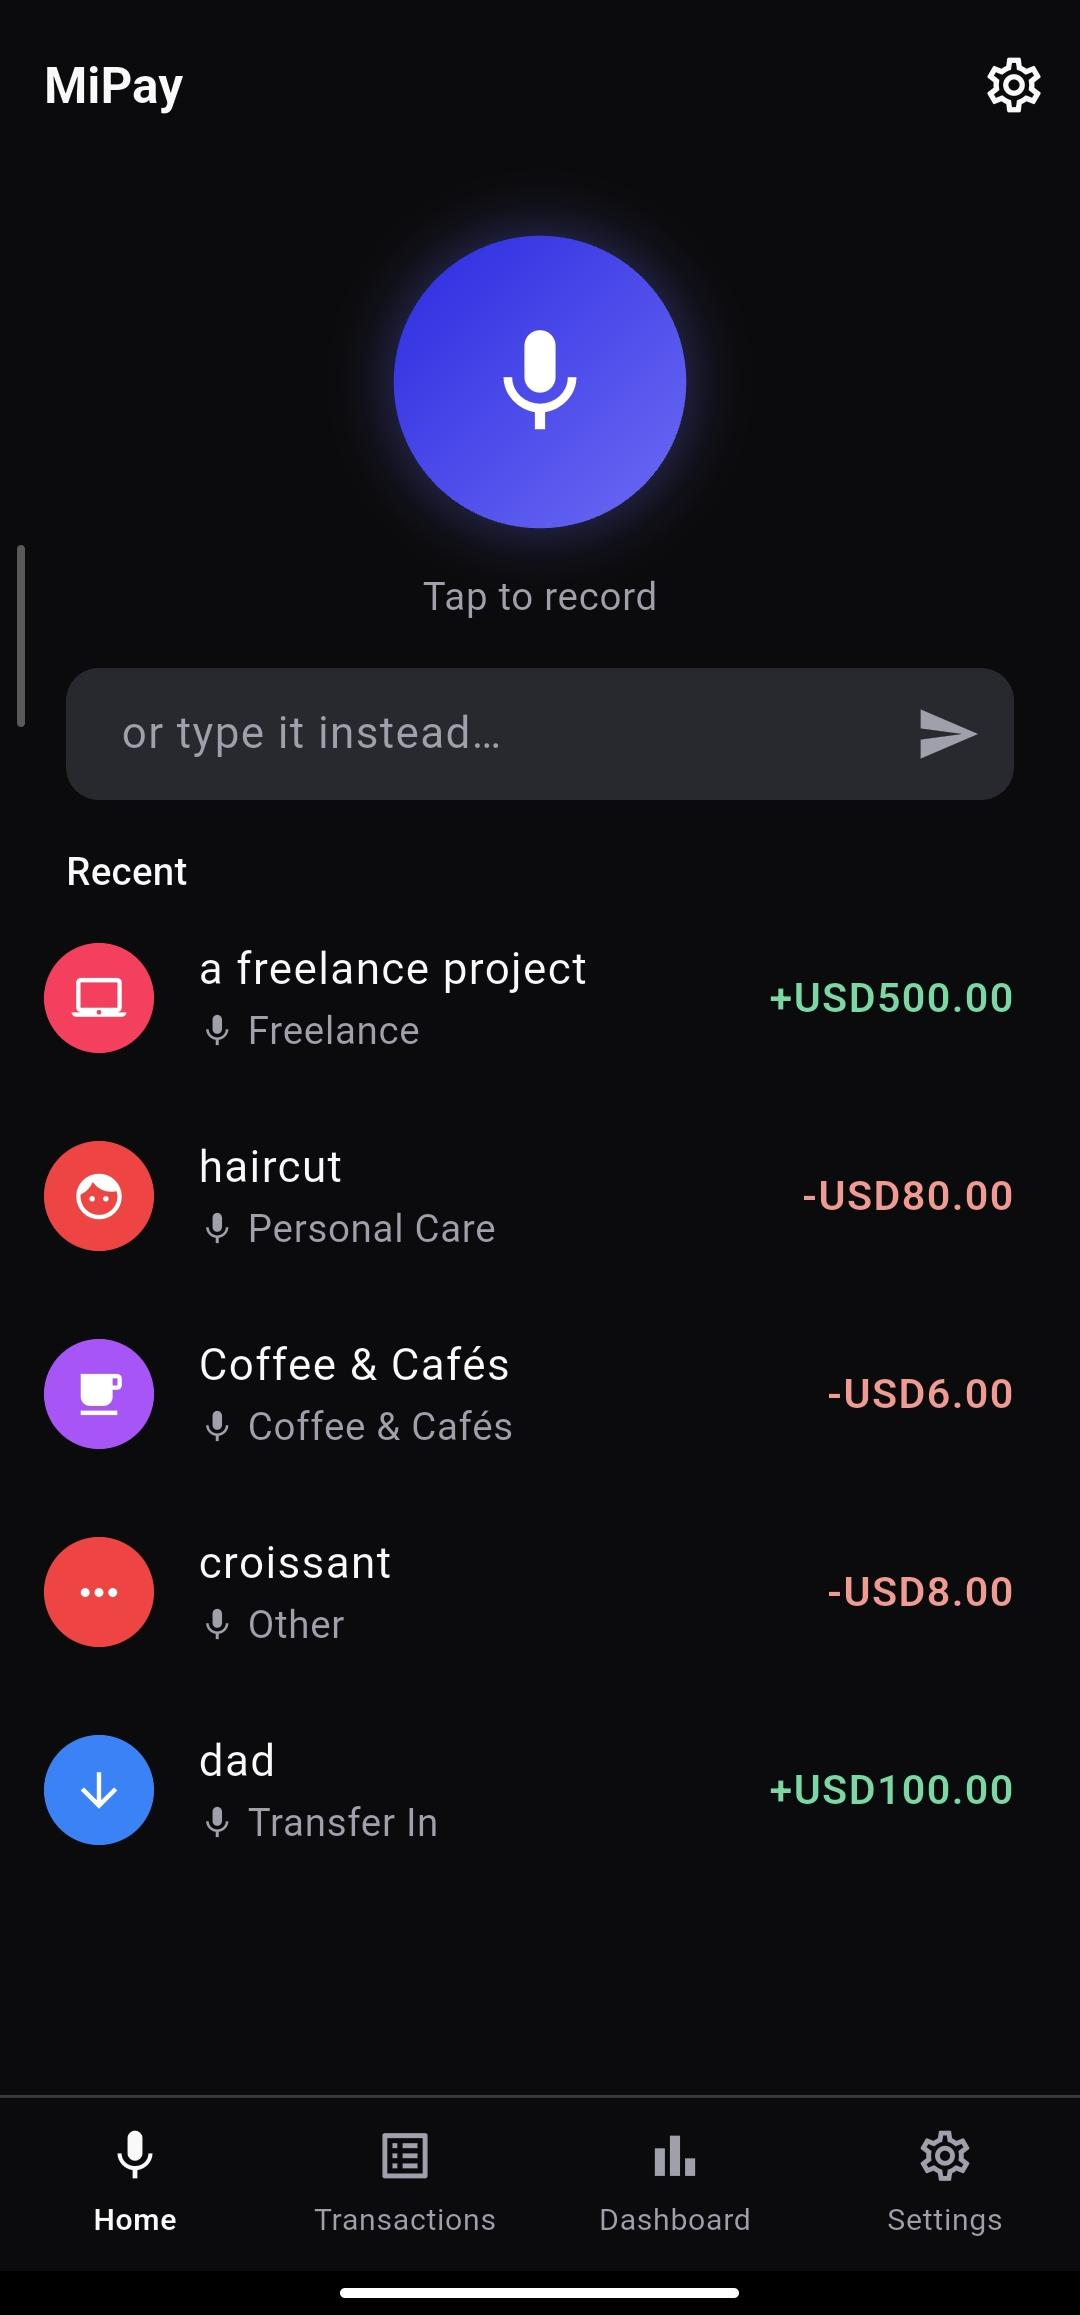
\includegraphics[width=0.32\textwidth]{figures/ui_home_record.jpg}\hfill
    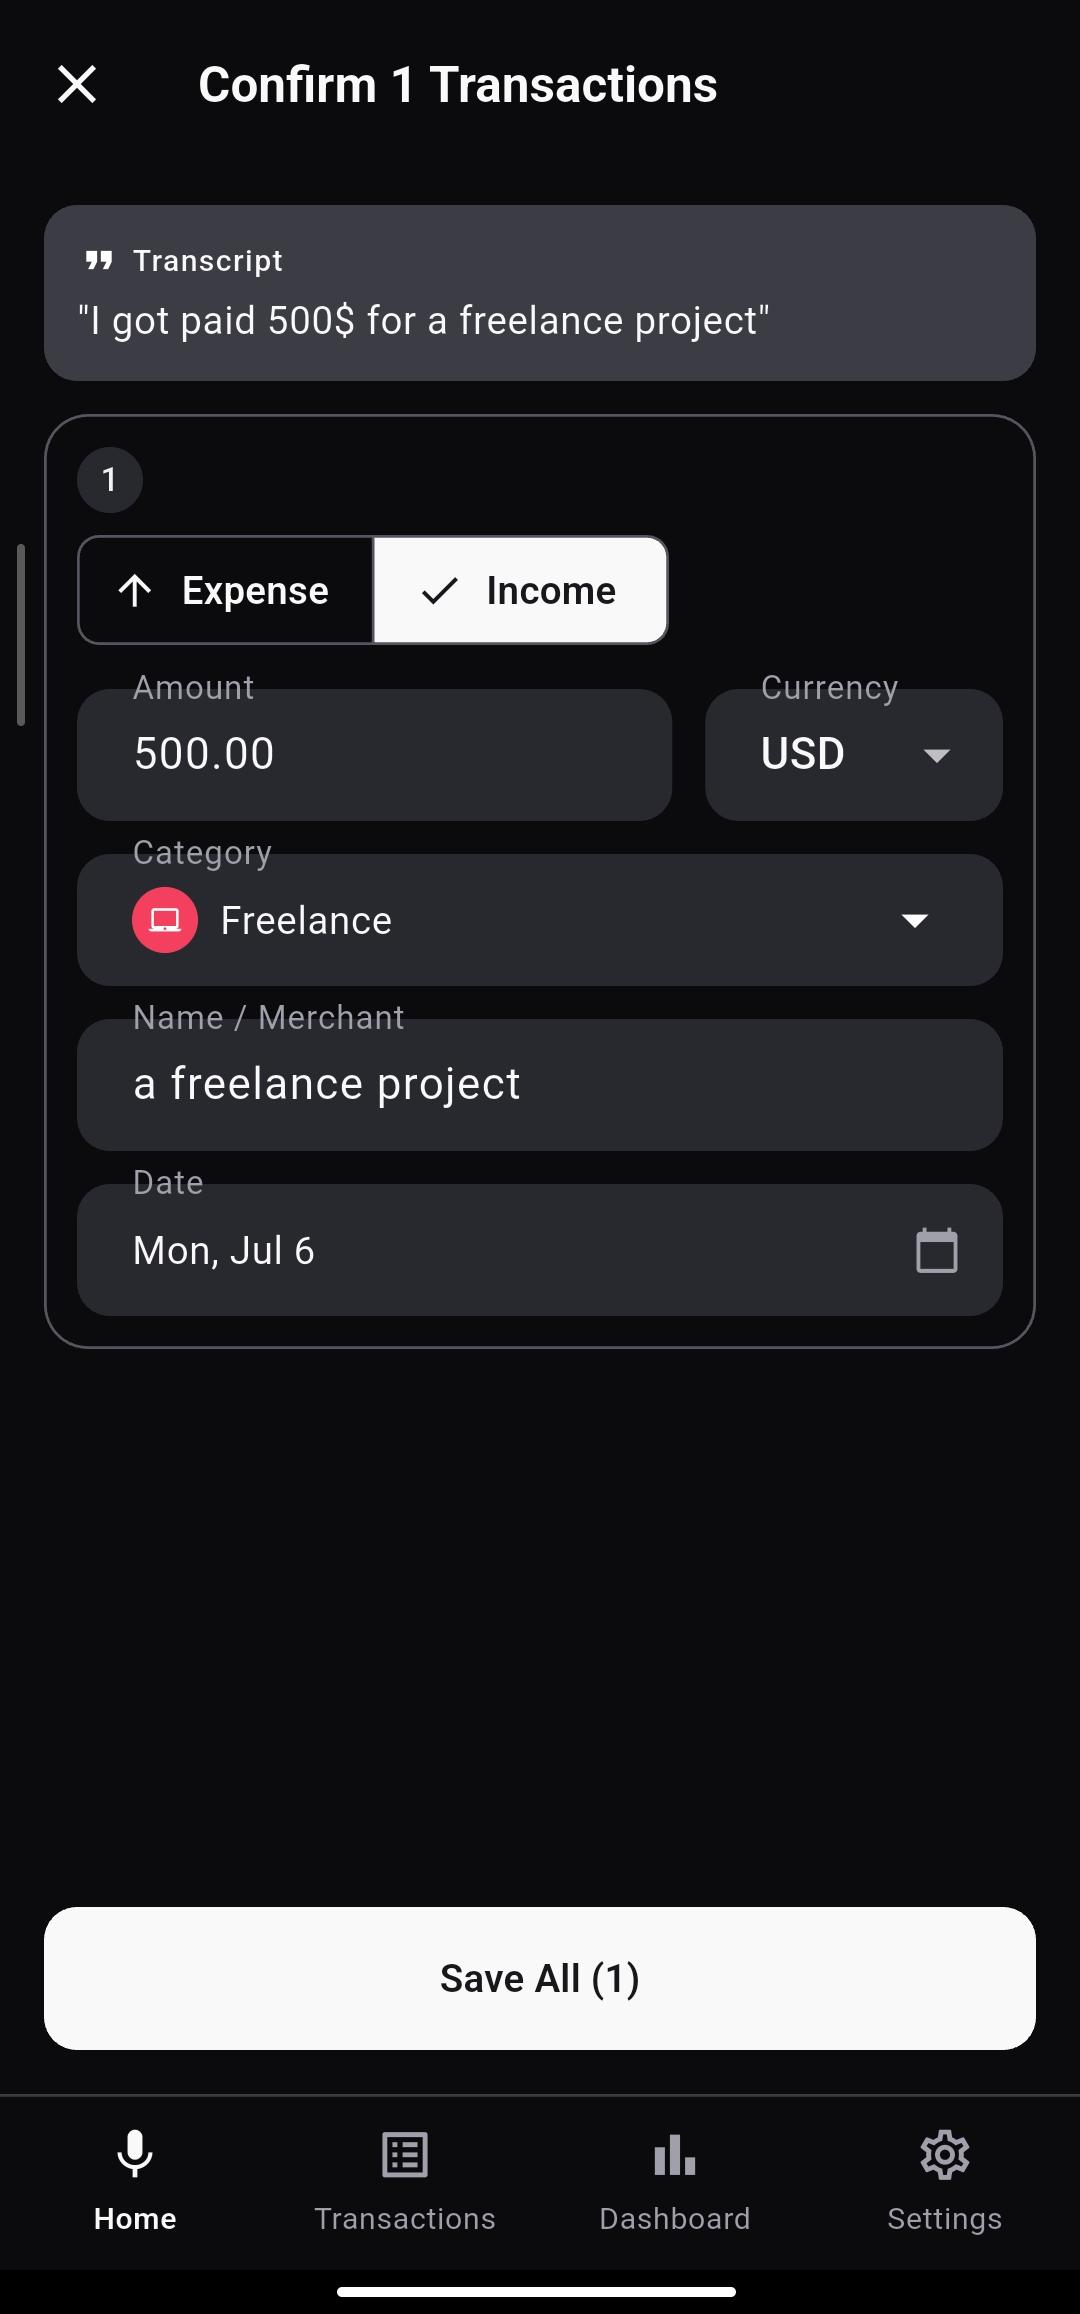
\includegraphics[width=0.32\textwidth]{figures/ui_confirm.jpg}
    \caption[Login, record, and confirm screens]{Left to right: the login screen;
    the home/record screen with its microphone button and monthly mini-summary; the
    confirmation screen showing one editable card per extracted transaction.}
    \label{fig:ui-1}
\end{figure}

\begin{figure}[H]
    \centering
    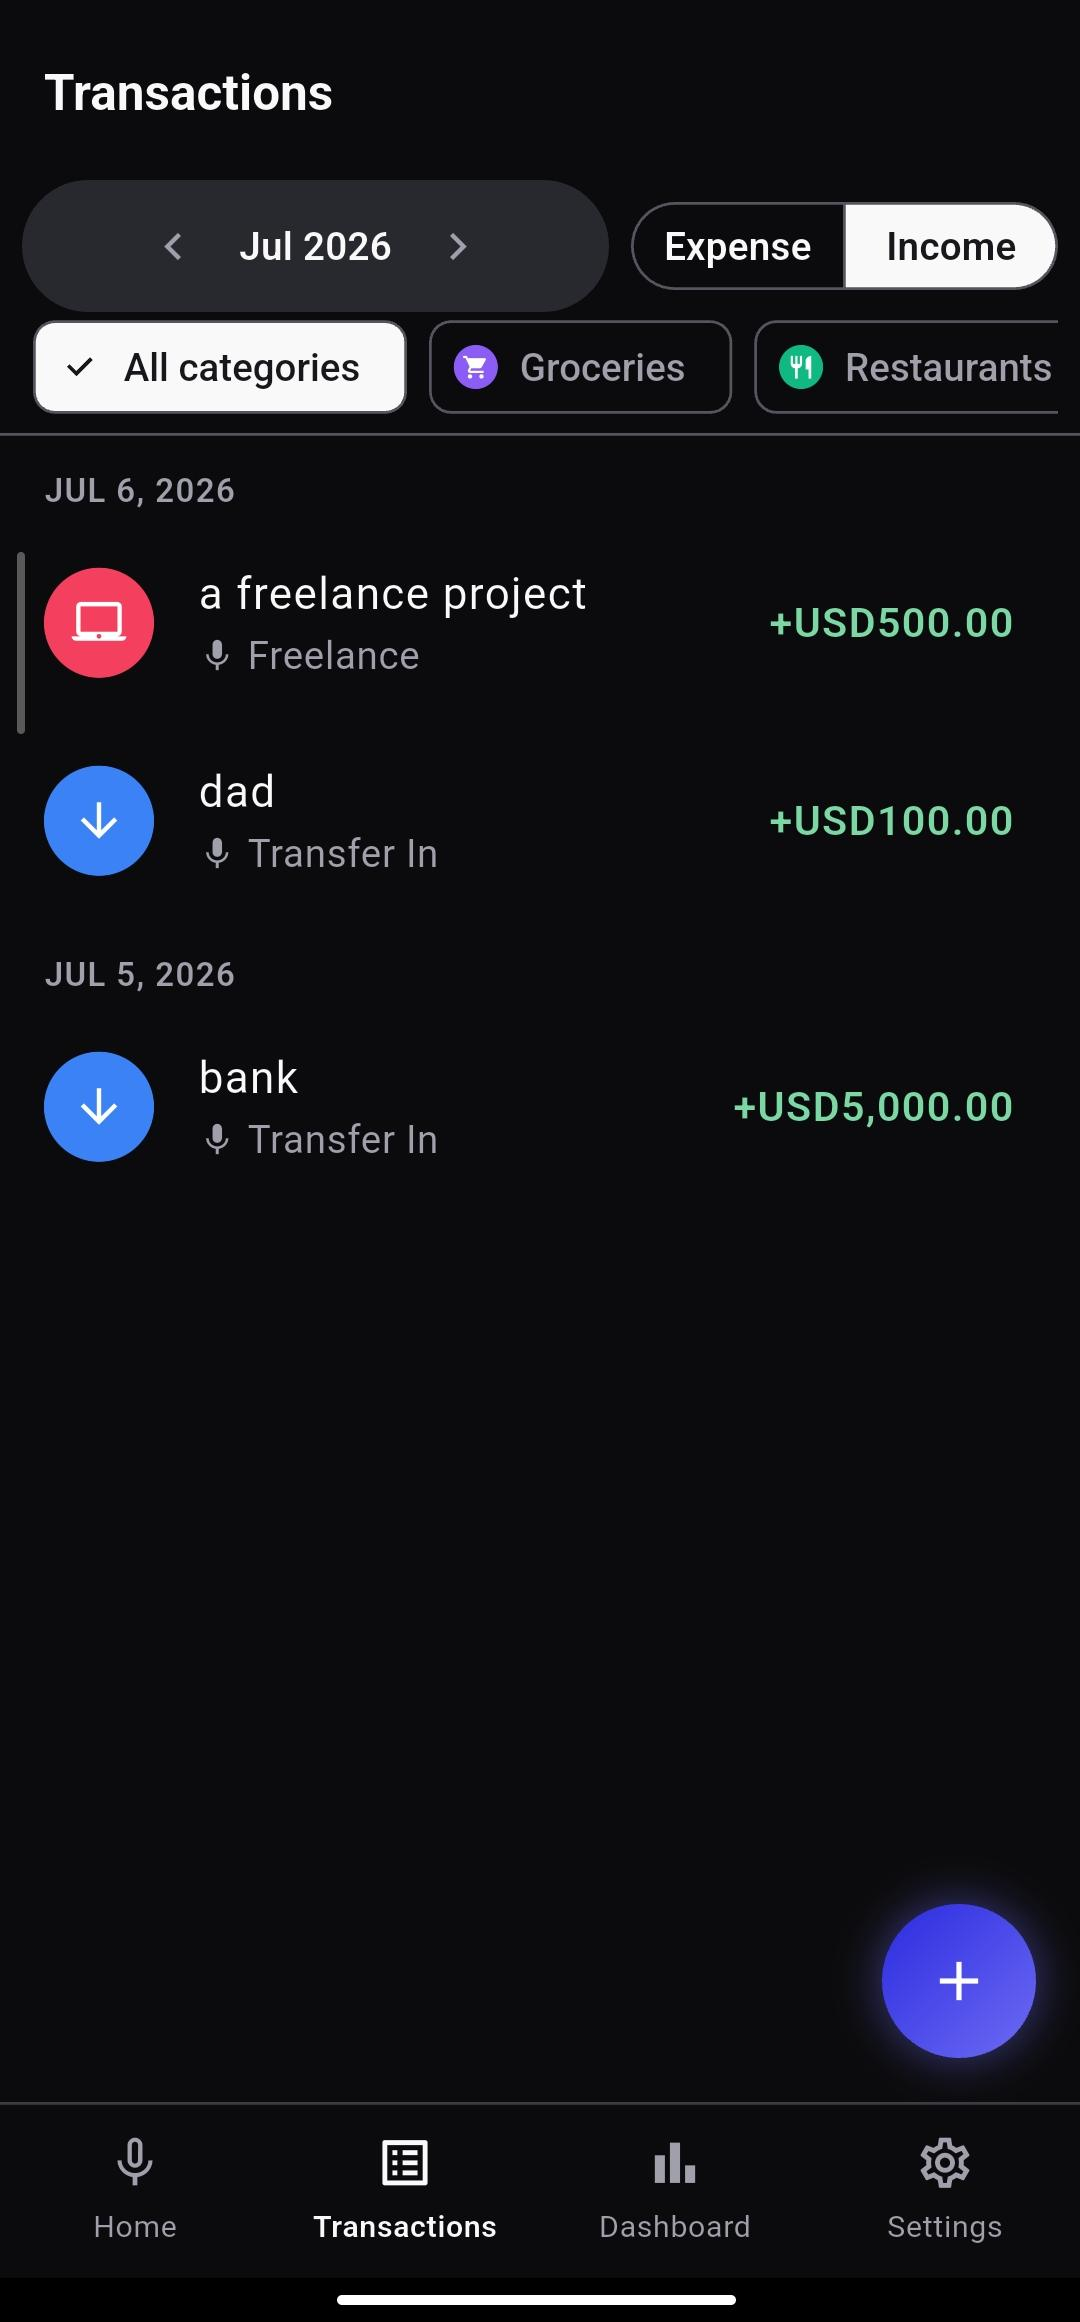
\includegraphics[width=0.32\textwidth]{figures/ui_transactions.jpg}\hfill
    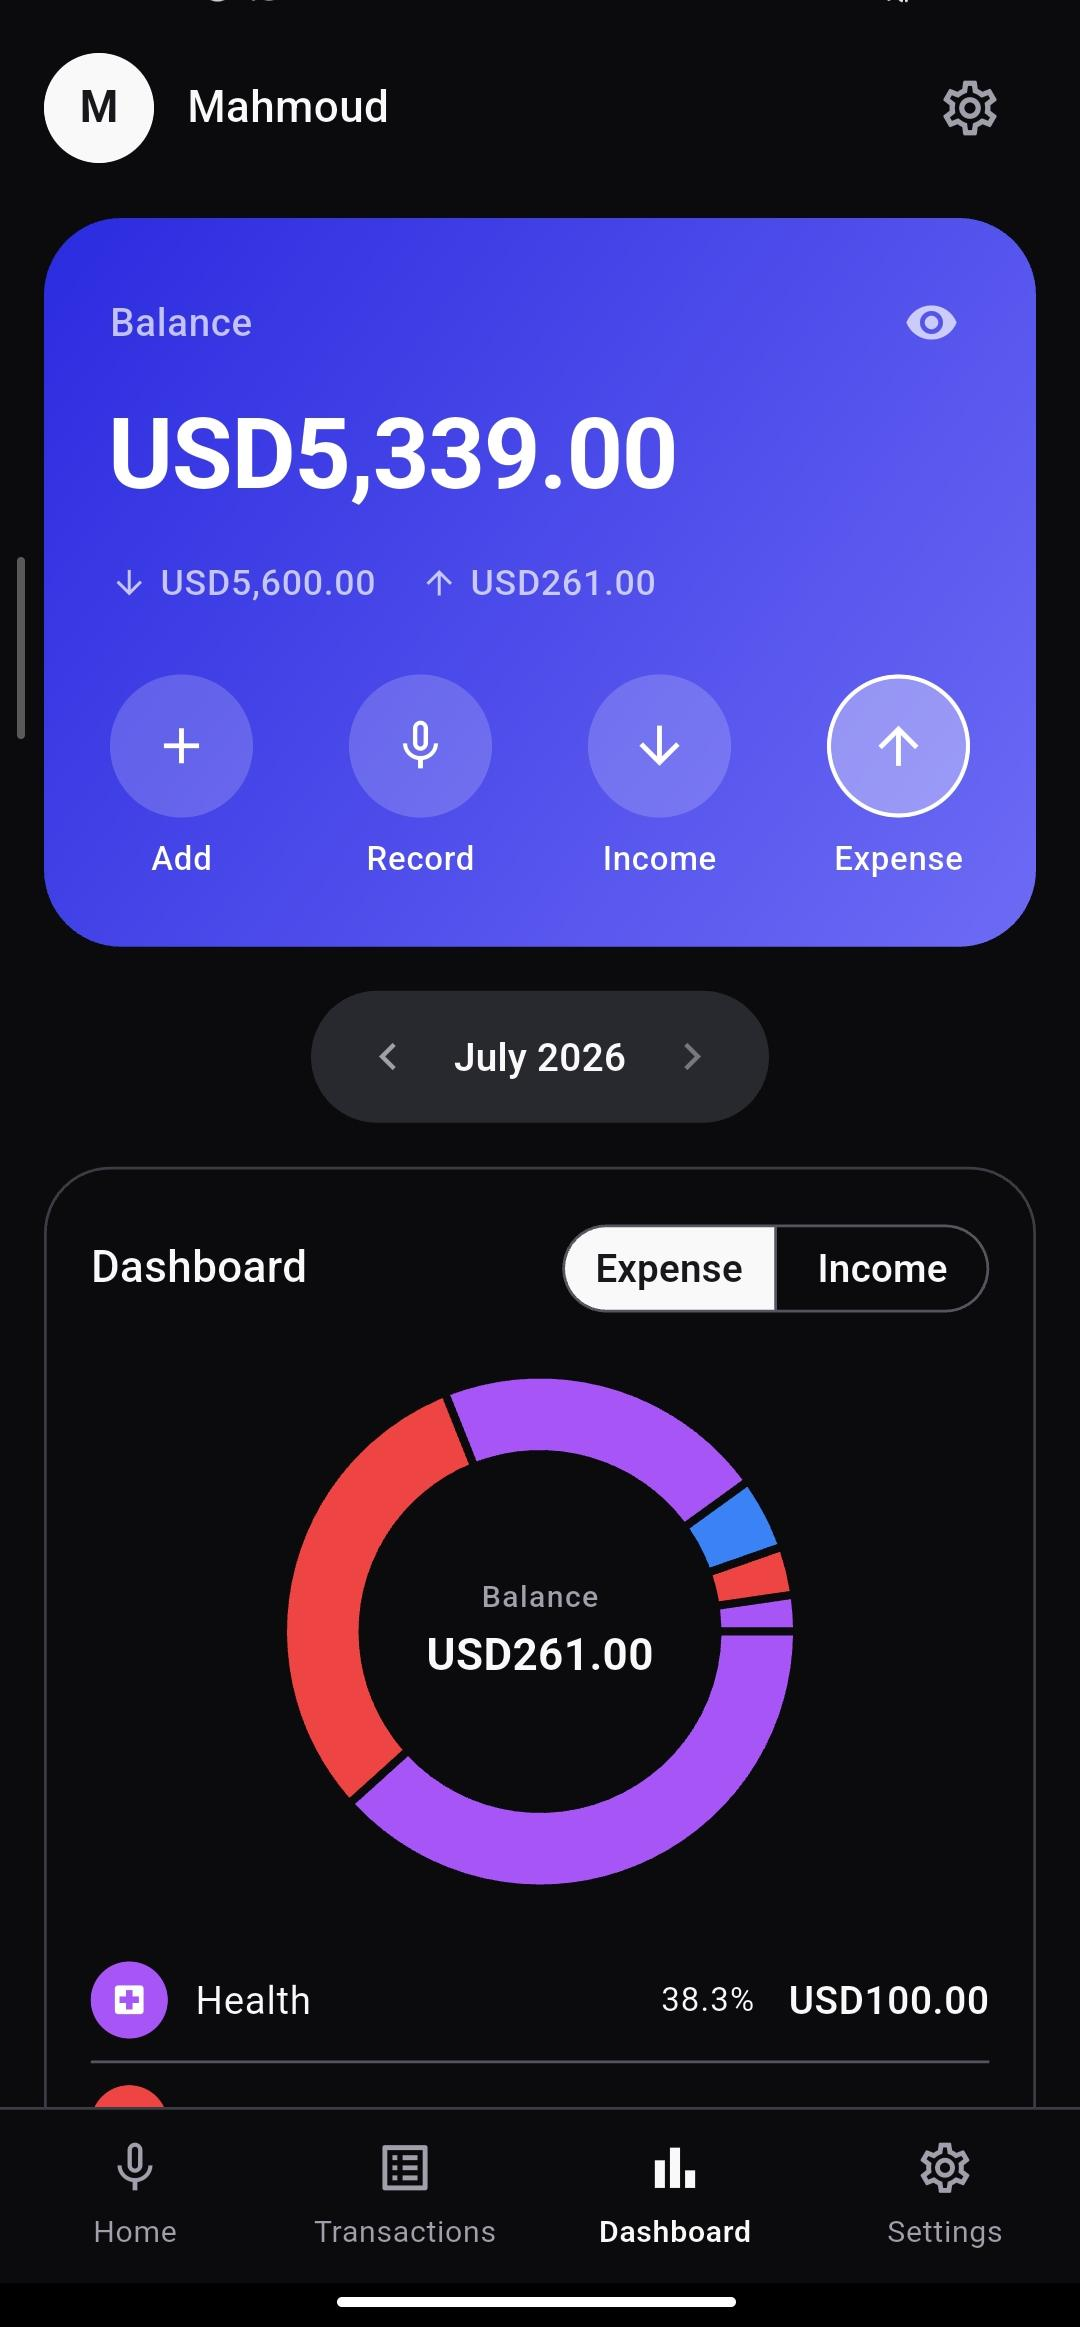
\includegraphics[width=0.32\textwidth]{figures/ui_dashboard.jpg}\hfill
    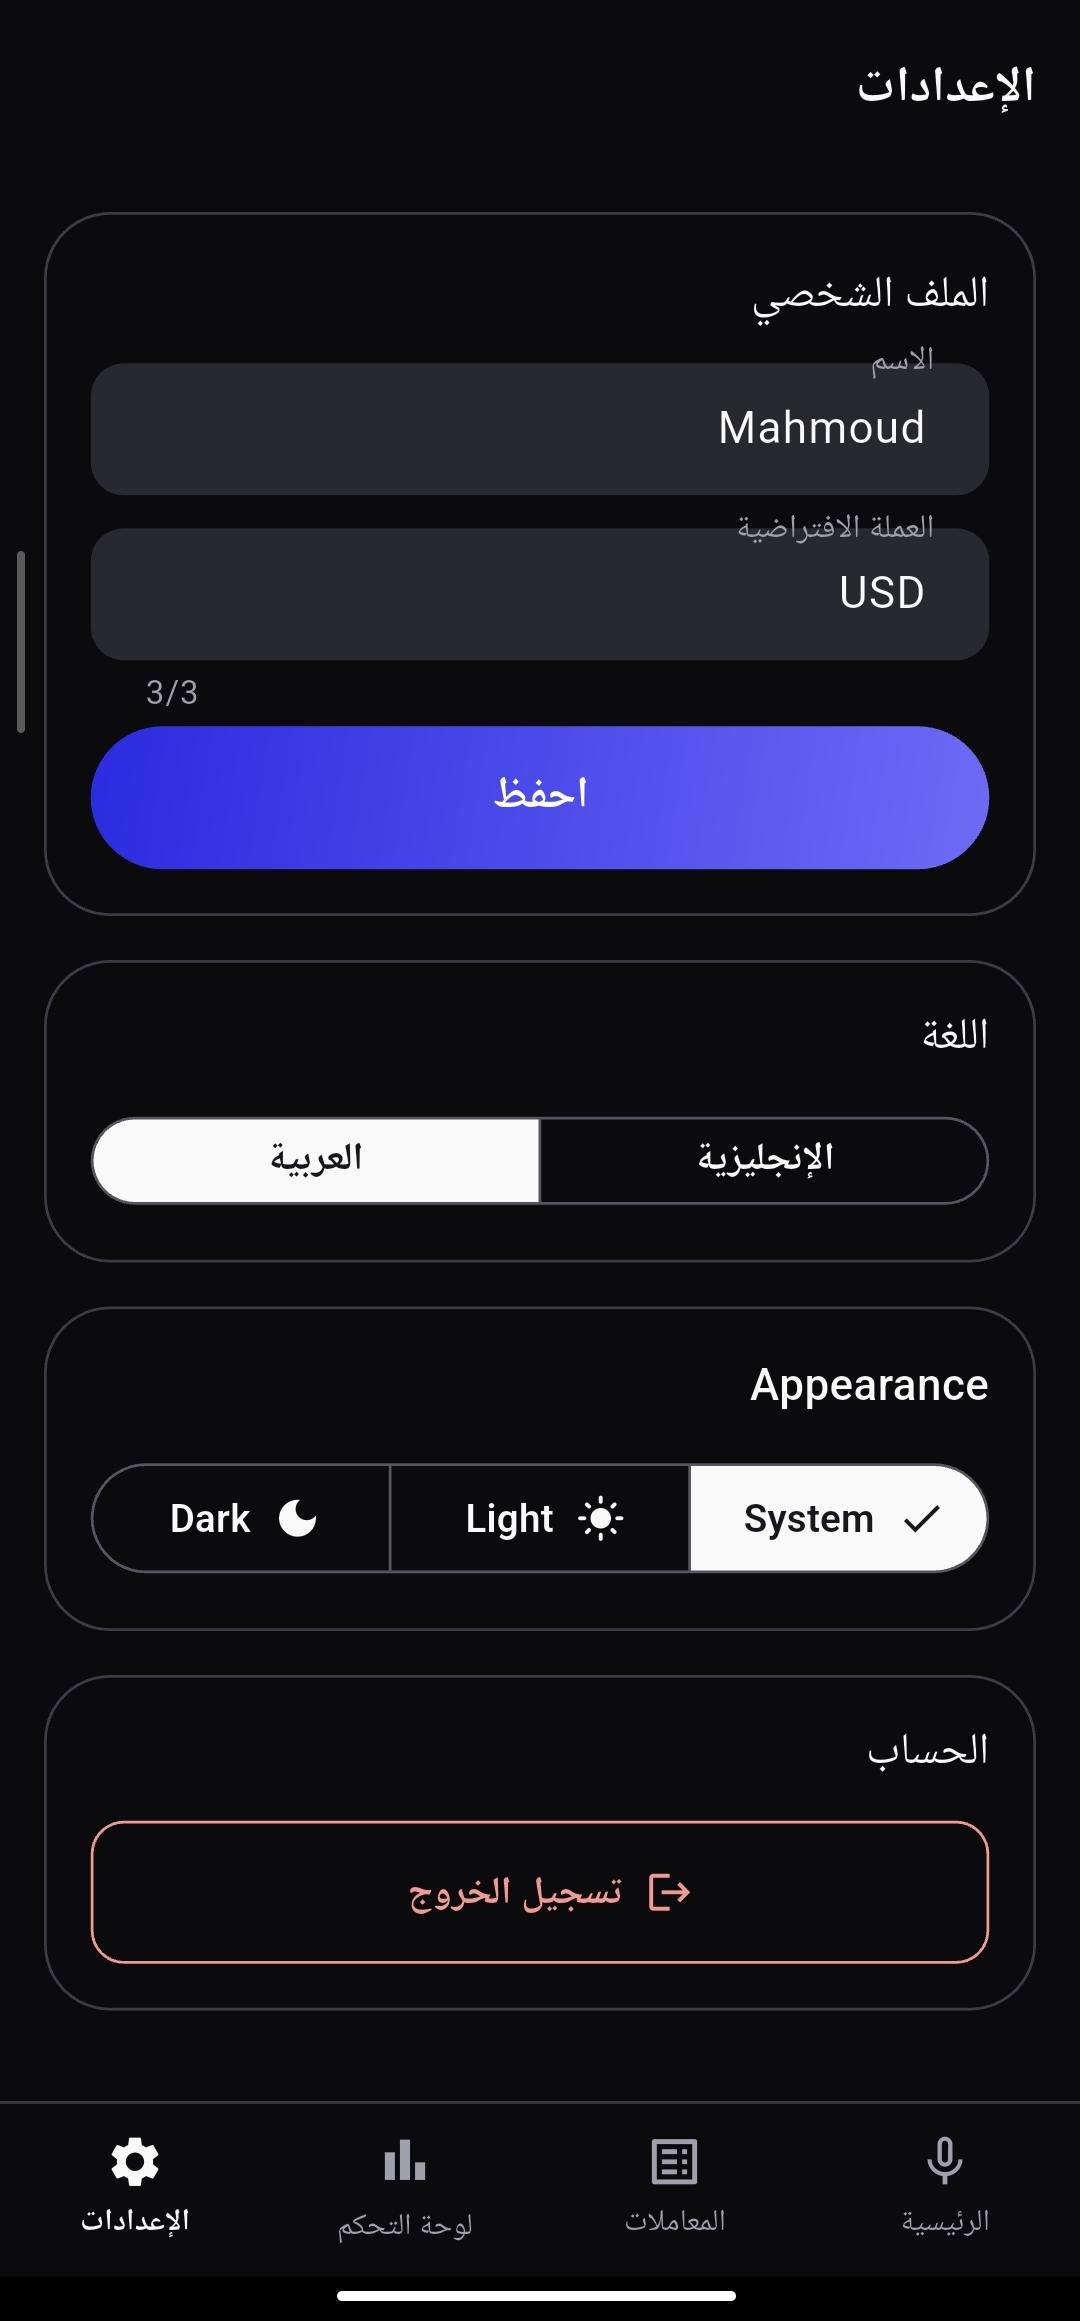
\includegraphics[width=0.32\textwidth]{figures/ui_settings_ar.jpg}
    \caption[Transactions, dashboard, and settings screens]{Left to right: the
    transactions list grouped by day with filters; the dashboard with stat cards
    and the category donut chart; the settings screen shown in Arabic
    (right-to-left) to demonstrate localization.}
    \label{fig:ui-2}
\end{figure}

\section{Implementation Challenges and Solutions}

\subsection{Technical Challenges Addressed}

\begin{table}[H]
\centering
\caption{Selected engineering challenges and their resolutions.}
\label{tab:challenges}
\small
\renewcommand{\arraystretch}{1.3}
\begin{tabularx}{\textwidth}{>{\raggedright\arraybackslash}p{4.2cm} X}
\toprule
\textbf{Challenge} & \textbf{Solution} \\
\midrule
Malformed JSON from the LLM & Schema-constrained decoding guarantees valid,
schema-conformant output, removing all JSON-repair logic. \\
Unreliable LLM date arithmetic & The LLM copies the raw date phrase; a
deterministic, tested resolver computes the absolute date. \\
Arabic-Indic numerals & A character-level normalization is applied before the LLM
and to the name field after. \\
Dialect date phrases missed by the parser & A pre-mapping table converts dialectal
forms to canonical phrases before parsing, with weekday retry transforms. \\
Multi-transaction utterances & A list-valued schema and few-shot examples that
demonstrate splitting; each record is post-processed independently. \\
Whisper hallucination on silence & Voice-activity-detection filtering trims silence
before transcription. \\
Per-request model loading latency & The Whisper model is a startup-loaded singleton;
transcription runs in a worker thread. \\
Token expiry mid-session & A Dio interceptor refreshes the access token once on a
401 and retries, otherwise logs out. \\
\bottomrule
\end{tabularx}
\end{table}

\subsection{Architecture Decisions}

Three decisions had outsized influence: the \emph{two-step save} (the AI endpoints
persist nothing, making errors harmless); the \emph{shared extraction core} (voice
and text modes differ only in the speech stage); and the \emph{fuzzy/exact split}
(the model understands, deterministic code computes). Each is documented in the
main text and is reflected directly in the module structure.

\section{Development Process and Quality Assurance}

\subsection{Development Methodology}

Development followed the phased milestone plan of the specification: scaffold,
authentication and database, transaction CRUD, the speech service, the extraction
pipeline, the voice UX, the dashboard and settings, the evaluation harness, and
hardening for demonstration. Each phase had explicit acceptance criteria.

\subsection{Performance Optimization}

Key optimizations include CTranslate2 \texttt{int8} inference for roughly four-fold
faster CPU transcription, the startup-loaded Whisper singleton, deterministic
(\texttt{temperature}\,$=0$) extraction for reproducibility, and database indexes on
\texttt{(user\_id, date)} and \texttt{(user\_id, category)} for the list and summary
queries.

\section{Technical Resources and Documentation}

\subsection{Source Code Repository}

The complete source---backend, mobile client, evaluation harness, dataset, and
Docker Compose configuration---resides in the project repository. The README
documents one-command setup; the specification and feature documents record the
design decisions referenced throughout this thesis.

\subsection{Additional Documentation}

The evaluation directory contains the labeled dataset, the speech and extraction
evaluation scripts, and the Arabic normalization utility, enabling third-party
reproduction of the results in Chapter~5.
